As \textit{Redes Neurais Convolucionais} (CNNs, do inglês \textit{Convolutional Neural Networks}) são modelos de redes neurais \emph{feedforward} com muitas camadas ocultas, em que cada camada possui uma finalidade específica e implementa uma determinada funcionalidade básica, como convolução, normalização, \textit{pooling}, etc \cite{ref:goodfellow,ref:khan}.

O funcionamento das CNNs reside especificamente na realização de operações de convolução. A \textit{convolução} é uma operação linear que calcula a soma dos produtos de toda a extensão de duas entradas em função de um determinado deslocamento, tendo como principal objetivo a extração de características da entrada por meio de um filtro, produzindo um  \textit{mapa de características} \cite{ref:goodfellow,ref:sewak}.

No contexto das CNNS, uma camada convolucional recebe um volume de entrada de $n$ dimensões e pode possuir um preenchimento  $p$ de zeros (\textit{zero-padding}), aplicado ao redor da entrada. Essa entrada é processada por $k$ filtros que representam os pesos e as conexões da CNN \cite{ref:khan}. Cada filtro consiste em uma matriz de números discretos e possui uma extensão espacial $e$, que é igual ao valor da altura e da largura do filtro, e um \textit{stride} $s$, que é a distância entre as aplicações de convolução consecutivas do filtro no volume de entrada \cite{ref:buduma}.

A Figura \ref{img:convolucao} exemplifica o processo de convolução aplicado em uma entrada de tamanho $5\times 5$ e \textit{zero-padding} $p = 1$. O filtro utilizado no exemplo possui extensão espacial $e = 2$ e \textit{stride} $s = 2$ com inicialização de pesos aleatória. É possível observar que o mapa de características é uma saída de tamanho $3\times 3$ em que cada um dos seus componentes é a da soma das multiplicações dos elementos do filtro com os elementos de um segmento da entrada \cite{ref:khan}.

\begin{figure}[!ht]
	\centering
  \caption{Exemplo de um processo de convolução aplicado em uma entrada de tamanho $5\times 5$ e um filtro de tamanho $2\times 2$. Fonte: \cite{ref:khan}.}
  \label{img:convolucao}
	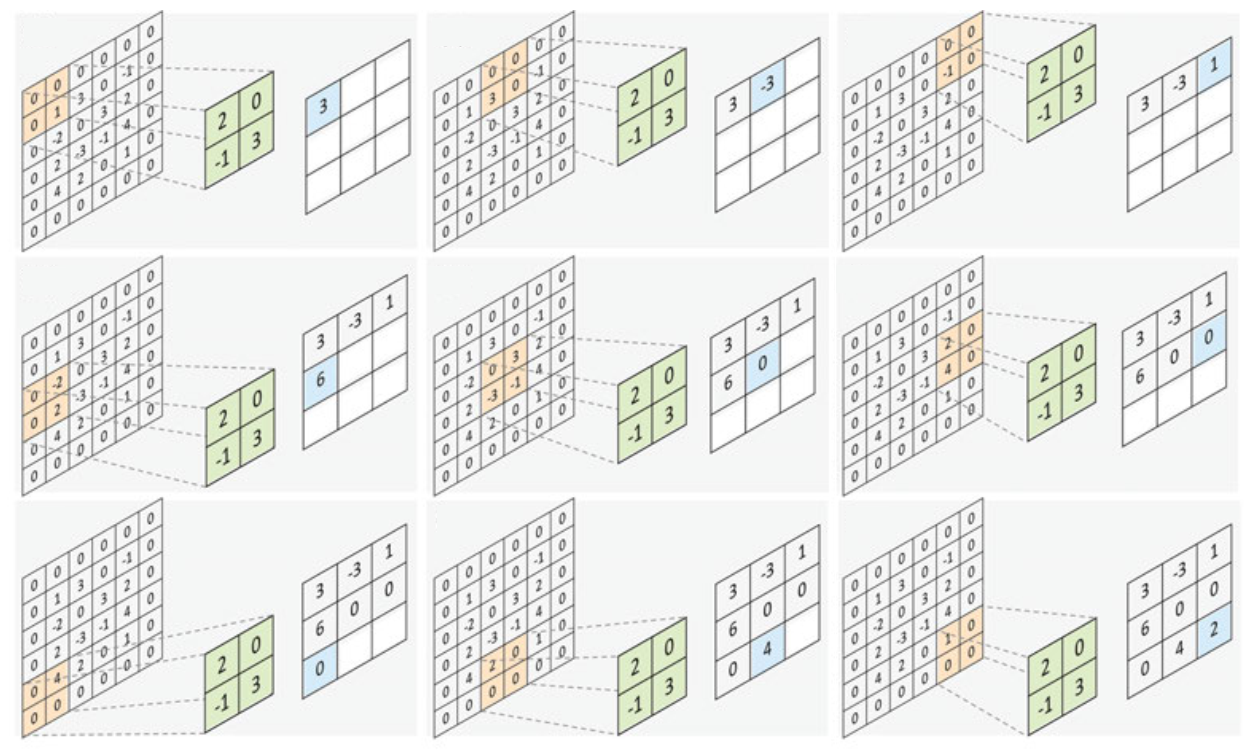
\includegraphics[width=0.9\textwidth]{./img/convolucao}
\end{figure}

No contexto de VC, em especial, em que as CNNs recebem imagens como entrada, as camadas de convolução atuam reconhecendo características visuais. As primeiras camadas convolucionais iniciam reconhecendo características mais simples, como linhas e bordas. Porém, à medida que a camada convolucional é mais profunda e que a entrada já passou por mapas de características mais elementares, é possível reconhecer características cada vez mais complexas, como texturas, objetos e até rostos, conforme ilustrado na Figura \ref{img:convolucao2}.

\begin{figure}[!ht]
	\centering
  \caption{Exemplo de mapas de características em uma CNN aplicados a um problema de classificação de imagens. Fonte: \cite{ref:khan}.}   \label{img:convolucao2}
	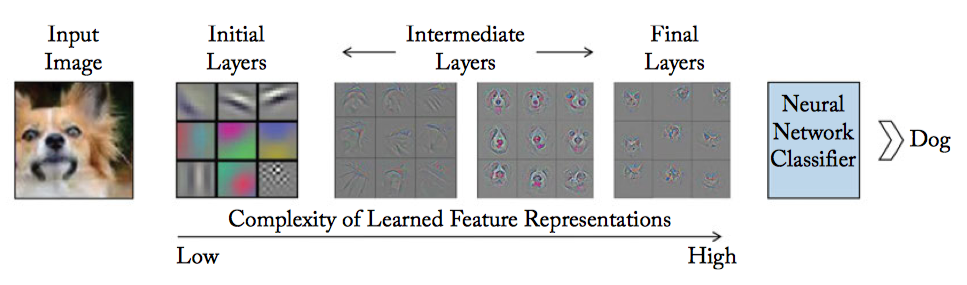
\includegraphics[width=0.9\textwidth]{./img/convolutions}
\end{figure}


Considerando a grande dimensionalidade dos dados, é preciso manter um número razoável de parâmetros ajustáveis, evitando uma sobrecarga de processamento. Assim, visando diminuir a dimensão dos mapas de características, tipicametne alternam-se camadas convolucionais e camadas de \textit{pooling}. Uma camada de \textit{pooling} é responsável por dividir o mapa de características recebido como entrada em blocos de tamanhos iguais, processando cada bloco para criar um mapa de características condensado. O processamento dos blocos é definido por uma função de \textit{pool} que pode ser, por exemplo, a função máximo, caracterizando o \emph{max-pooling} \cite{ref:buduma,ref:khan}.

As últimas camadas de uma CNN normalmente são as \textit{Fully Connected Layers} (FCL), ou camadas completamente conectadas, as quais correspondem essencialmente às camadas de convolução que utilizam filtros de tamanho $1 \times$ 1 em que cada elemento é densamente conectado à todos os elementos da camada anterior \cite{ref:khan}. Nesta última camada, adota-se tipicamente a função de ativação \textit{softmax}, também chamada de função exponencialmente normalizada, a qual escala o vetor de saída em um vetor de probabilidades, recurso muito útil em problemas de classificação  \cite{ref:JAI-2017}. O processo de aprendizagem utilizado pelas FCL é baseado nos conceitos das RNAs do tipo MLP e no algoritmo de treinamento \textit{backpropagation} \cite{ref:gulli, ref:khan}. A Figura \ref{img:convolucao3} sintetiza a ideia da disposição das camadas em uma CNN.

\begin{figure}[!ht]
	\centering
  \caption{Disposição de camadas em uma CNN. Fonte: \cite{ref:gulli}.}   \label{img:convolucao3}
	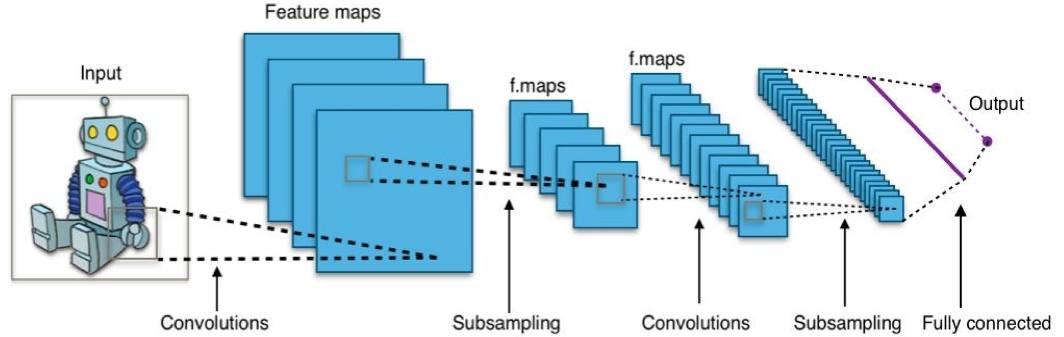
\includegraphics[width=0.9\textwidth]{./img/cnn}
\end{figure}

Durante o processo de treinamento, as CNNs utilizam técnicas de regularização para  evitar possíveis erros de generalização, tais como o \emph{overfiting}  \cite{ref:goodfellow}.  Uma das abordagens mais populares para isto consiste na técnica de \emph{Dropout}, a qual temporariamente evita a propagação de alguns pesos da rede mediante uma probabilidade $p$. Intuitivamente, a existência de \emph{Dropout} força a CNN a ser acurada mesmo na ausência de certa informação \cite{ref:buduma}. A utilização de camadas do tipo \textit{Dropout} impacta positivamente de forma significativa no desempenho das CNNs na fase de testes, prevendo a saída associada a exemplos previamente não conhecidos \cite{ref:khan}.
